\subsection{M.PD.1 - Percentuale di requisiti obbligatori soddisfatti}

\begin{figure}[H]
    \centering
    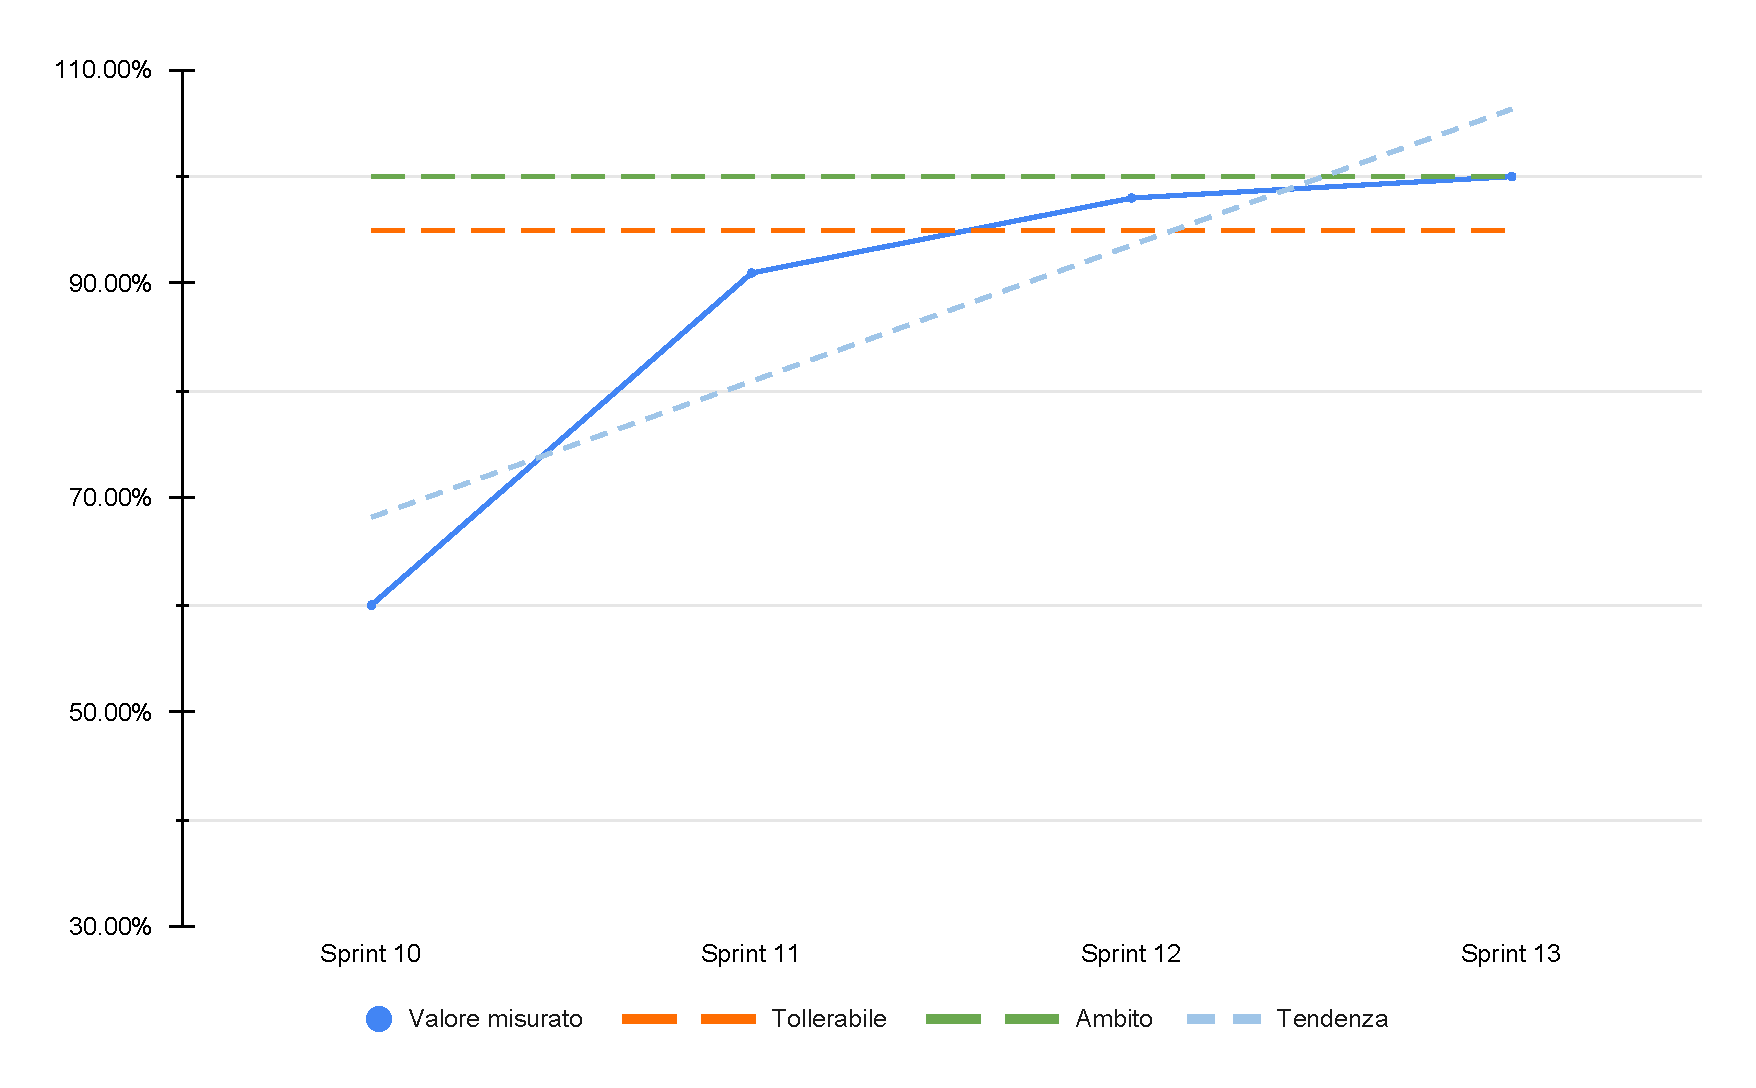
\includegraphics[width=\textwidth]{assets/requisiti_obbligatori_soddisfatti.pdf}
    \caption{M.PD.1 - Percentuale di requisiti obbligatori soddisfatti}
\end{figure}

\par Nei primi due sprint della \glossario{PB}, il team ha raggiunto un buon livello di copertura dei requisiti obbligatori, pur rimanendo al di sotto della soglia tollerabile. Nonostante i rapidi progressi nello sviluppo del \glossario{front-end}, l'assenza di un'architettura \glossario{back-end} ben definita non consentiva il completo soddisfacimento dei requisiti. Dopo l'implementazione del modello architetturale e la configurazione dei test, il gruppo è riuscito a ottenere una copertura adeguata dei requisiti obbligatori. La piena copertura dei requisiti è stata infine raggiunta durante lo \glossario{sprint} 13.